\documentclass[11pt]{report}
% Paquetes esenciales
\usepackage[utf8]{inputenc}
\usepackage[T1]{fontenc}
\usepackage[spanish]{babel}
\usepackage{amsmath, amssymb, amsthm}
\usepackage{tikz}
\usepackage{xcolor}
\usepackage{csquotes}
\usepackage[most]{tcolorbox}
\usepackage{hyperref}  % Enlaces internos
\usepackage{graphicx}  % Para incluir imágenes
\usepackage{geometry}  % Márgenes más cómodos
\usepackage[numbers]{natbib} % Bibliografía
\usepackage{pdfpages}
\geometry{left=3cm, right=3cm, top=3cm, bottom=3cm}

% Comandos renombrados o nuevos
\newcommand{\x}{\textbf{x}}

% widehat y widecheck
\DeclareFontFamily{U}{mathx}{}
\DeclareFontShape{U}{mathx}{m}{n}{<-> mathx10}{}
\DeclareSymbolFont{mathx}{U}{mathx}{m}{n}
\DeclareMathAccent{\widecheck}{0}{mathx}{"71}
\renewcommand{\check}{\widecheck}
\renewcommand{\hat}{\widehat}
\renewcommand{\check}{\widecheck}

% norma 3 lineas
\newcommand{\seminorm}[1]{{\left\vert\kern-0.25ex\left\vert\kern-0.25ex\left\vert #1 
    \right\vert\kern-0.25ex\right\vert\kern-0.25ex\right\vert}}

% norma alargada
\newcommand{\norm}[1]{\left\lVert#1\right\rVert}

% Definir colores personalizados para las cajas
\definecolor{mygrayback}{RGB}{245, 245, 245}
\definecolor{mygrayframe}{RGB}{80, 80, 80}
\definecolor{mygrayframeproof}{RGB}{140, 140, 140}

% Redefinir el ambiente de Teorema
\newtcolorbox[auto counter, number within=section]{theorem}[2][]{%
  colback=mygrayback, colframe=mygrayframe, fonttitle=\bfseries,
  title=Teorema~\thetcbcounter: #2,#1, breakable}

% Redefinir el ambiente de Lema
\newtcolorbox[auto counter, number within=section]{lemma}[2][]{%
  colback=mygrayback, colframe=mygrayframe, fonttitle=\bfseries,
  title=Lema~\thetcbcounter: #2,#1, breakable}

% Redefinir el ambiente de Proposición
\newtcolorbox[auto counter, number within=section]{proposition}[2][]{%
  colback=mygrayback, colframe=mygrayframe, fonttitle=\bfseries,
  title=Proposición~\thetcbcounter: #2,#1, breakable}

% Redefinir el ambiente de Nota
\newtcolorbox[auto counter, number within=section]{note}[2][]{%
  colback=mygrayback, colframe=mygrayframe, fonttitle=\bfseries,
  title=Nota~\thetcbcounter: #2,#1, breakable}

% Redefinir el ambiente de Corolario
\newtcolorbox[auto counter, number within=section]{corollary}[2][]{%
  colback=mygrayback, colframe=mygrayframe, fonttitle=\bfseries,
  title=Corolario~\thetcbcounter: #2,#1, breakable}

% Redefinir el ambiente de Ejemplo
\newtcolorbox[auto counter, number within=section]{example}[2][]{%
  colback=mygrayback, colframe=mygrayframe, fonttitle=\bfseries,
  title=Ejemplo~\thetcbcounter: #2,#1, breakable}

% Redefinir el ambiente de Definición
\newtcolorbox[auto counter, number within=section]{definition}[2][]{%
  colback=mygrayback, colframe=mygrayframe, fonttitle=\bfseries,
  title=Definición~\thetcbcounter: #2,#1, breakable}

% Redefinir el ambiente de Notación
\newtcolorbox[auto counter, number within=section]{notation}[2][]{%
  colback=mygrayback, colframe=mygrayframe, fonttitle=\bfseries,
  title=Notación~\thetcbcounter: #2,#1, breakable}

% Eliminar la definición original de \proof
\let\proof\relax
\let\endproof\relax

% Redefinir el ambiente de Demostración (sin usar caracteres especiales en la clave)
\newtcolorbox{proof}[1][]{%
  colback=mygrayback, colframe=mygrayframeproof, fonttitle=\bfseries,
  title=Demostración, #1, breakable}

% Redefinir el ambiente de Solución
\newtcolorbox{solution}[1][]{%
  colback=mygrayback, colframe=mygrayframeproof, fonttitle=\bfseries, title=Solución,#1, breakable}



\pagestyle{fancyplain}% <- use fancyplain instead fancy
\fancyhf{}
\fancyhead[R]{\thepage}
\renewcommand{\headrulewidth}{0pt}
\setlength{\headheight}{14pt}

\usepackage{natbib}
\bibliographystyle{plainnat}

\begin{document}

\pagenumbering{roman} 

\begin{titlepage}
\centering
{\bfseries\LARGE Universidad Nacional de Colombia \par}
\vspace{1cm}
{\scshape\Large Facultad de Ciencias \par}
\vspace{3cm}
{\scshape\Huge Algunas notas de análisis númerico \par}
\vfill
{\Large Andrés David Cadena Simons \par}
\vfill
{\Large \today \par}
\end{titlepage}

\tableofcontents

\doublespacing
\pagenumbering{arabic} 

\chapter{Introduction}
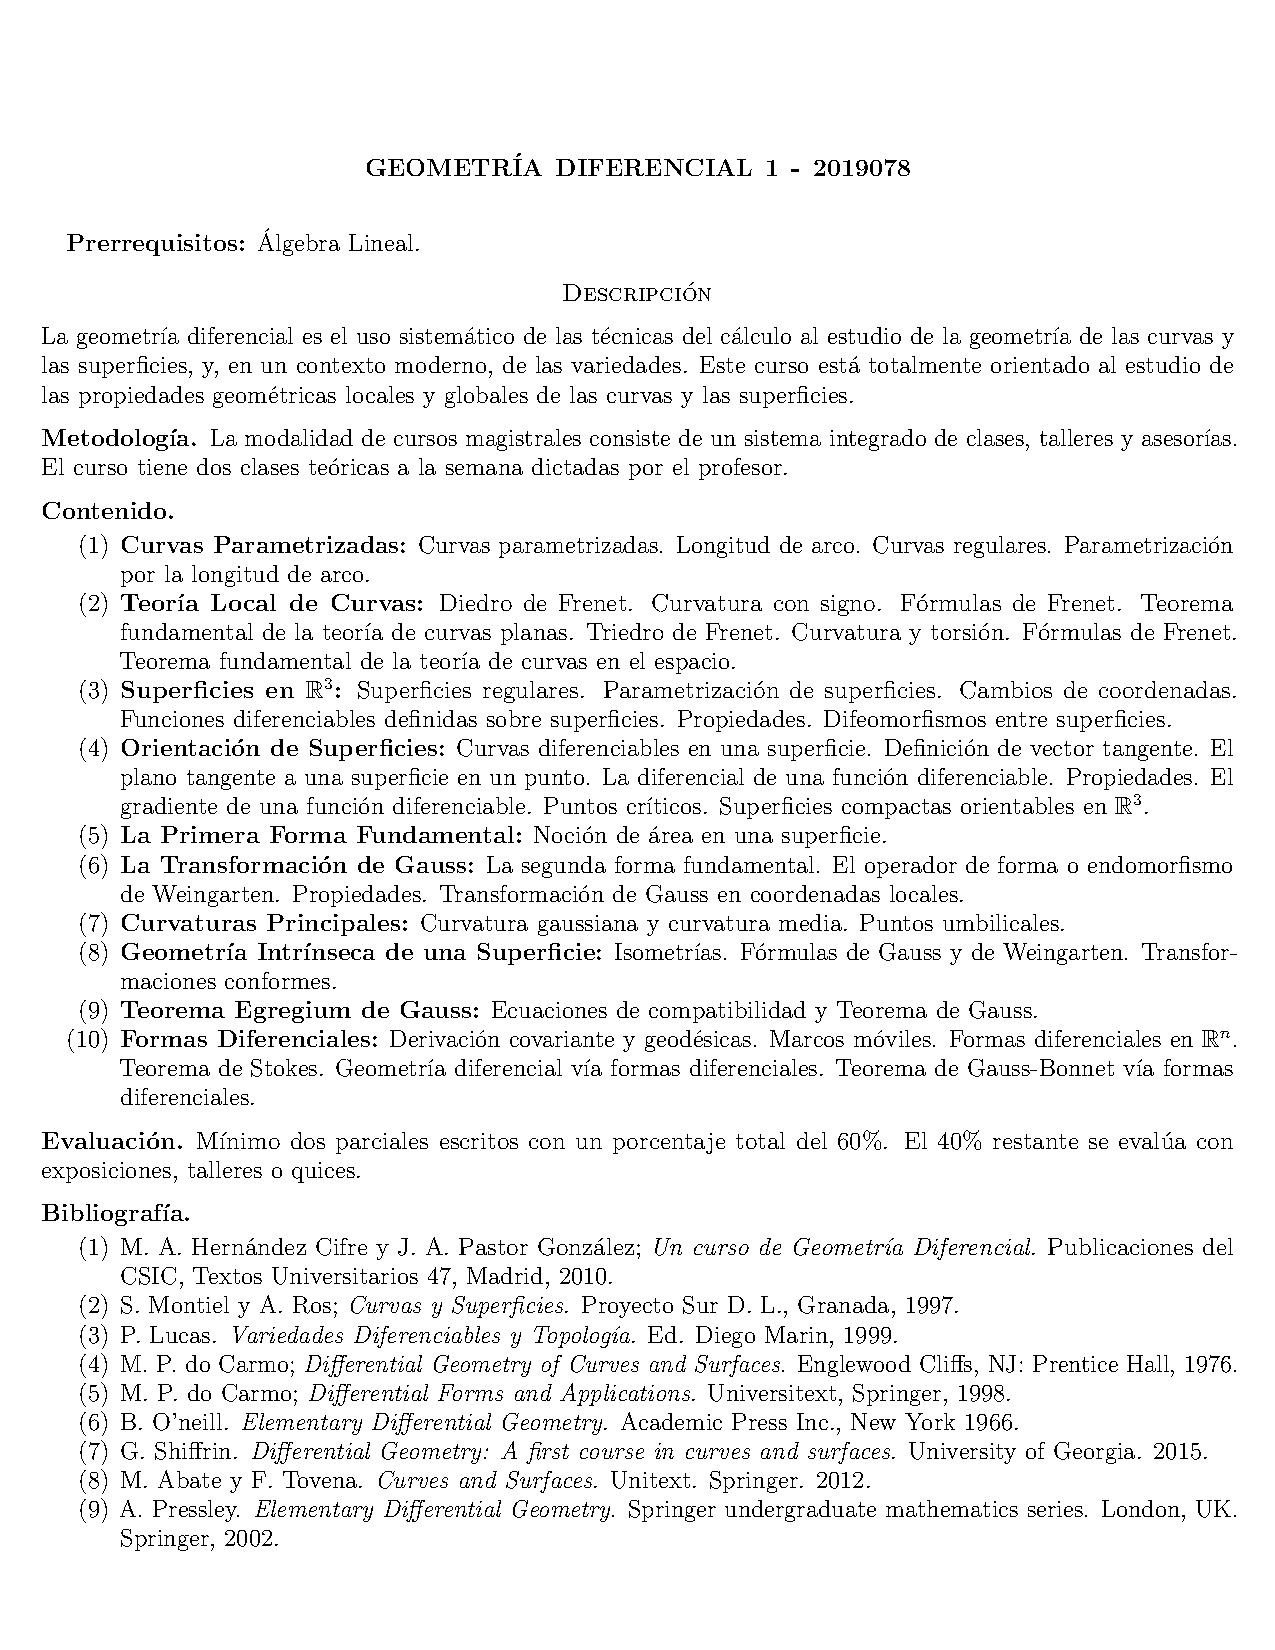
\includepdf[pages=-, fitpaper=true]{ProgramaGeoDif1.pdf}
\begin{itemize}
  \item Datos de la profesora.
  \item Calificación.
    \begin{itemize}
      \item $\%25$ Parcial I.
      \item $\%25$ Parcial II.
      \item $\%10$ Asistencia.
      \item $\%40$ Póster final. 
    \end{itemize}
\end{itemize}


\chapter{Teoría de aproximación.}
Este capitulo hablará sobre problemas de mínimos cuadrados, está totalmente basado en el libro \cite{MR2597943} con un par de comentarios o ejercicios propuestos por mi o por la clase. 
\newpage
\section{Problemas de mínimos cuadrados.}
  \subsection{Aproximación por mínimos cuadrados discretos.}
Considere el problema de calcular los valores de una función en puntos no tabulados, dados los datos experimentales en la siguiente tabla:
\begin{center}
  \begin{tabular}{|c|c|}
    \hline
    $x_i$ & $y_i$\\
    \hline 
    $1$ & $1.3$\\
    $2$ & $3.5$\\
    $3$ & $4.2$\\
    $4$ & $5.0$\\
    $5$ & $7.0$\\
    $6$ & $8.8$\\
    $7$ & $10.1$\\
    $8$ & $12.5$\\
    $9$ & $13.0$\\
    $10$ & $15.6$\\
    \hline
  \end{tabular}
\end{center}
La siguiente figura muestra una gráfica de los valores de la tabla:
\begin{center}
  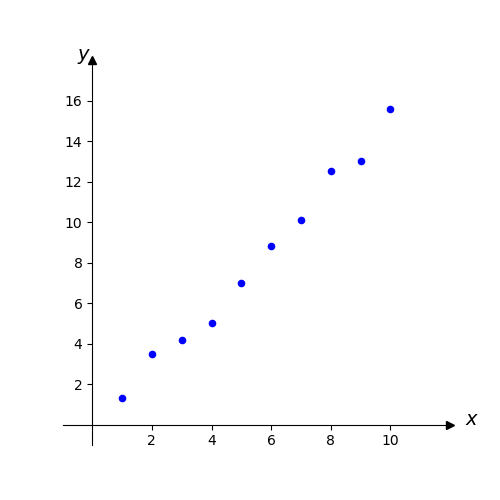
\includegraphics[scale=0.7]{chapters/chapter02/scripts/tabla.png}  
\end{center}
A partir de esta gráfica, parece que la relación real entre $x$ y $y$ es lineal. La razón probable para que ninguna linea se ajuste con precisión a los datos son los errores en estos últimos. Por lo que es poco razonable solicitar que la función de aproximación concuerde exactamente con los datos. De hecho, dicha función introduciría oscilaciones que no estaban presentes originalmente. Por ejemplo, la gráfica del polinomio de interpolación de noveno grado para los datos de la tabla se verán en la siguiente figura:
\begin{center}
  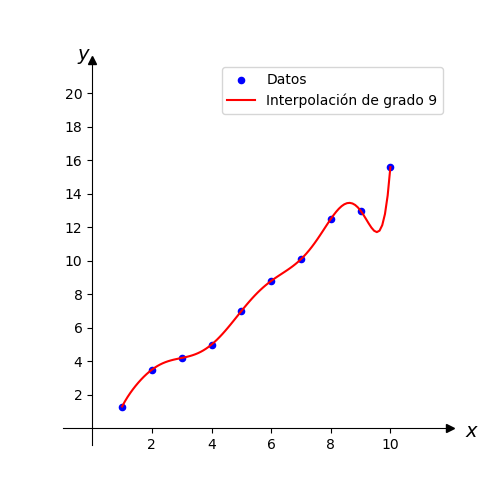
\includegraphics[scale=1]{chapters/chapter02/scripts/tabla-interpolacion.png}
\end{center}
Este polinomio es claramente una predicción de la información entre una serie de puntos de datos. Un mejor enfoque seria encontrar la recta que se aproxima “mejor” (en cierto sentido), incluso si no concuerda precisamente con los datos en ningún punto.\\
Sea que $a_1x_i+a_0$ denota el $i$-ésimo valor en la recta de aproximación y que $y_i$ es el $i$-ésimo valor de $y$ dado. Suponemos que las variables independientes, las $x_i$, son exactas; son las variables dependientes, las $y_i$, de las que sospechamos. Esto es una suposición razonable en muchas situaciones experimentales.\\
El problema de encontrar la ecuación de la mejor aproximación lineal en el sentido
absoluto requiere encontrar los valores $a_0$ y $a_1$ para minimizar:
\begin{align*}
  E_{\infty}(a_0,a_1)=\max_{1\leq i\leq 10}\{y_i-(a_1x_i+a_0)\}.
\end{align*}
Normalmente esto recibe el nombre de problema minimáx y no es posible manejarlo con técnicas fundamentales.\\
Otro enfoque para determinar la mejor aproximación lineal implica encontrar los valores de $a_0$ y $a_1$ para minimizar: 
\begin{align*}
  E_1(a_0,a_1)=\sum_{i=1}^{10}|y_i-(a_1x_i+a_0)|.
\end{align*}
Esta cantidad recibe el nombre de \textbf{desviación absoluta}. Para minimizar una función de dos variables, necesitamos igualar sus derivadas parciales a cero y resolver simultáneamente las ecuaciones resultantes. En el caso de la desviación absoluta, necesitamos encontrar $a_0$ y $a_1$ con:
\begin{align*}
  0=\frac{\partial }{\partial a_0}\sum_{i=1}^{10}|y_i-(a_1x_i+a_0)|\hspace{0.2cm}y\hspace{0.2cm}0=\frac{\partial }{\partial a_1}\sum_{i=1}^{10}|y_i-(a_1x_i+a_0)|.
\end{align*}
El problema es que la función valor absoluto no es diferenciable en cero y podríamos no encontrar soluciones para este par de ecuaciones.
\subsubsection{Mínimos cuadrados lineales.}
  El enfoque de mínimos cuadrados para este problema implica determinar la mejor linea de aproximación cuando el error relacionado es la suma de los cuadrados de las diferencias entre los valores $y$ en la linea de aproximación y los valores $y$ proporcionados. Por lo tanto, deben encontrarse las constantes $a_0$ y $a_1$ que minimizan el error de mínimos cuadrados:
  \begin{align*}
    E_2(a_1,a_0)=\sum_{i=1}^{10}[y_i-(a_1x_i+a_0)]^2.
  \end{align*}
  El método de mínimos cuadrados es el procedimiento mas conveniente para determinar mejores aproximaciones lineales, pero también hay consideraciones técnicas importantes que lo favorecen. En general, mientras el enfoque minimáx asigna demasiado peso a un bit de datos con un gran error, el método de desviación absoluta no da suficiente peso a un punto que esté fuera de la linea con la aproximación. El enfoque de mínimos cuadrados asigna considerablemente mas peso en un punto que esta fuera de la linea que al resto de los datos, pero no permitir que el punto domine por completo la aproximación. Una razón adicional para considerar el enfoque de mínimos cuadrados implica el estudio de la distribución estadística del error. 
  El problema general de ajustar la mejor linea de mínimos cuadrados para una recopilación de datos $\{x_i,y_i\}_{i=1}^{m}$, implica minimizar el error total,
  \begin{align*}
    E\equiv E_{2}(a_0,a_1)=\sum_{i=1}^{m}[y_i-(a_1x_i+a_0)]^{2},
  \end{align*}
  respecto a los parámetros $a_0$ y $a_1$. Para que se presente un mínimo, necesitamos que:
  \begin{align*}
    \frac{\partial E}{\partial a_0}=0\hspace{0.2cm}y\hspace{0.2cm}\frac{\partial E}{\partial a_1}=0,
  \end{align*}
  es decir,
  \begin{align*}
    0=-2\sum_{i=1}^{m}(y_i-a_1x_i-a_0)
  \end{align*}
  y
  \begin{align*}
    0=-2\sum_{i=1}^{m}(y_i-a_1x_i-a_0)(x_i)
  \end{align*}
  Estas ecuaciones zzz


\chapter{Aproximación de valores propios.}
Este capitulo hablará sobre problemas de factorización, está totalmente basado en el libro \cite{MR2597943} con un par de comentarios o ejercicios propuestos por mi o por la clase. 
\section{Método de Householder}
En la siguiente sección usaremos el método QR para reducir una matriz tridiagonal simétrica en una matriz similar que es casi diagonal. Las entradas diagonales de la matriz reducida son aproximaciones para los valores propios de la matriz dada. En esta sección presentamos un método concebido por Alston Householder para reducir una matriz simétrica arbitraria en una matriz tridiagonal similar. A pesar de que existe una conexión entre los problemas que estamos resolviendo en estas dos secciones, el método de Householder tiene una aplicación tan amplia en áreas diferentes a la aproximación de valores propios que merece un trato especial.\\
El método de Householder se usa para encontrar una matriz tridiagonal $B$ que es similar a una matriz simétrica $A$ determinada. El teorema 9.16 (\cite{MR2597943}) implica que $A$ es similar a la matriz diagonal $D$, ya que existe una matriz ortogonal $Q$ con la propiedad de que $D=Q^{-1}AQ$. Puesto que, en general, la matriz $Q$ (y por consiguiente, $D$) es difícil de calcular, el método de Householder ofrece un compromiso. Después de haber implementado el método de Householder, es posible usar métodos eficientes, como el algoritmo QR, para aproximar con exactitud los valores propios de la matriz tridiagonal simétrica resultante.
\subsection{Transformaciones de Householder.}
\begin{definition}{}
  Sea $w\in\mathbb{R}^{n}$ con $w^{T}w=1$. Entonces la matriz $n\times n$:
  \begin{align*}
    P=I-2ww^T
  \end{align*}
  recibe el nombre de \textbf{transformación Householder}.
\end{definition}
Las transformaciones de Householder se usan para los bloques externos de entradas cero en vectores o columnas de matrices de manera en extremo estable respecto al error de redondeo. Las propiedades de las transformaciones se dan en el siguiente teorema.
\begin{theorem}{}
  Si una tranformación de Householder, $P=I-2ww^{T}$, es simetrica y ortogonal, entonces $P^{-1}=P$.
\end{theorem}
\begin{proof} 
  Note que
  \begin{align*}
    (ww^{T})^{T}=(w^T)^Tw^T&=ww^T,
  \end{align*}
  luego:
  \begin{align*}
    P^T&=(I-2ww^{T})^T\\
    &=I^{T}-2(ww^{T})^T\\
    &=I-2ww^{T}\\
    &=P.
  \end{align*}
  Además, como $w^{T}w=1$ se satisface que:
  \begin{align*}
    PP^T&=(I-2ww^T)(I-2ww^T)\\
    &=I-2ww^T-2ww^{T}+4ww^Tww^T\\
    &=I-4ww^T+4ww^T &&\text{Ya que $w^Tw=1$.}\\
    &=I.
  \end{align*}
  Así $P^{-1}=P^T=P$.
\end{proof}
El método de Householder comienza determinando una transformación $P^{(1)}$ tal que $A^{(2)}=P^{(1)}AP^{(1)}$ tiene entradas ceros fuera de la primera columna de $A$, comenzando con la tercera fila, es decir:
\begin{equation}\label{eq:m-householder-1}
  a_{j1}^{(2)}=0 \hspace{1cm}\text{Para cada $j=3,4,\cdots,n$.}
\end{equation}
Por simetría también tenemos $a_{1j}^{(2)}=0$.\\
Ahora seleccionamos un vector $w=(w_1,w_2,\cdots,w_n)^{T}$ de tal forma que $w^Tw=1$, la ecuación $\ref{eq:m-householder-1}$ se mantiene y en la matriz:
\begin{align*}
  A^{(2)}&=P^{(1)}AP^{(1)},\\
  &=(I-2ww^T)A(I-2ww^T),
\end{align*}
tenemos $a_{11}^{(2)}=a_{11}$ y $a_{j1}^{(2)}=0$ para cada $j=3,4,\cdots,n$. Esta selección impone $n$ condiciones en los $n$ valores desconocidos $w_1,w_2,\cdots,w_n$.\\
Al establecer $w_1=0$ garantizamos que $a_{11}^{(2)}=a_{11}$. Queremos:
\begin{align*}
  P^{(1)}=I-2ww^T,
\end{align*}
para satisfacer:
\begin{equation}\label{eq:m-householder-2}
  P^{(1)}(a_{11},a_{21},a_{31},\cdots,a_{n1})^{T}=(a_{11},\alpha,0,\cdots,0)^T
\end{equation}
donde $\alpha$ se seleccionará más adelante. Para simplificar la notación, si:
\begin{align*}
  \hat{w}=(w_2,w_3,\cdots,w_n)^{T}\in\mathbb{R}^{n-1}, \hat{y}=(a_{21},a_{31},\cdots,a_{n1})^{T}\in\mathbb{R}^{n-1},  
\end{align*}
y $\hat{P}$ es una transformación de Householder $(n-1)\times(n-1)$:
\begin{align*}
  \hat{P}=I_{n-1}-2\hat{w}\hat{w}^T.
\end{align*}
Entonces la ecuación $\ref{eq:m-householder-2}$ se convierte en:\\
Inserte matrices feas\\ 
con:
\begin{equation}\label{eq:m-householder-9.10}
  \hat{P}\hat{y}=(I_{n-1}-2\hat{w}\hat{w}^T)\hat{y}=\hat{y}-2(\hat{w}^T\hat{y})\hat{w}=(\alpha,0,\cdots,0)^T.
\end{equation}
Sea $r=\hat{w}^T\hat{y}$. Entonces:
\begin{align*}
  (\alpha,0,\cdots,0)^{T}=(a_{21}-2rw_2,a_{31}-2rw_3,\cdots,a_{n1}-2rw_n)^T,
\end{align*}
y podemos determinar todas las $w_i$ una vez que conocemos $\alpha$ y $r$. Al equiparar los componentes da:
\begin{align*}
  \alpha=a_{21}-2rw_2
\end{align*}
y
\begin{align*}
  0=a_{j1}-2rw_j, \hspace{1cm}\text{para cada }j=3,4\cdots,n.
\end{align*}
Por lo tanto:
\begin{equation}\label{eq:m-householder-9.11}
  2rw_2=a_{21}-\alpha,
\end{equation}
y
\begin{equation}\label{eq:m-householder-9.12}
  2rw_j=a_{j1},\hspace{1cm}\text{para cada }j=3,4,\cdots,n.
\end{equation}
Al elevar al cuadrado ambos lados de cada una de las ecuaciones \ref{eq:m-householder-9.11}, \ref{eq:m-householder-9.12} y sumar los términos correspondientes da:
\begin{align*}
  4r^2\sum_{j=2}^{n}w_j^2=(a_{21}-\alpha)^{2}+\sum_{j=3}^{n}a_{j1}^{2}
\end{align*}
note que como $ww^{T}=1$ y $w_1=0$, entonces $\sum_{j=2}^{n}w_{j}^{2}=1$,
\begin{equation}\label{eq:m-householder-9.13}
  4r^{2}=\sum_{j=2}^{n}a_{j1}^{2}-2\alpha a_{21}+\alpha^2.
\end{equation}
La ecuación \ref{eq:m-householder-9.10} y el hecho de que $P$ es ortogonal implica que:
\begin{align*}
  \alpha^2&=(\alpha,0,\cdots,0)(\alpha,0\cdots,0)^{T},\\
  &=(\hat{P}\hat{y})^{T}\hat{P}\hat{y},\\
  &=\hat{y}^{T}\hat{P}^{T}\hat{P}\hat{y},\\
  &=\hat{y}^T\hat{y}.
\end{align*}
Por lo tanto:
\begin{align*}
  \alpha^{2}=\sum_{j=2}^{n}a_{j1}^{2},
\end{align*}
lo que, al sustituir en la ecuación \ref{eq:m-householder-9.13}, da
\begin{align*}
  2r^{2}=\sum_{j=2}^{n}a_{j1}^2-\alpha a_{21}.
\end{align*}
Para garantizar $2r^2=0$ si y sólo si $a_{21}=a_{31}=\cdots=a_{n1}=0$ seleccionamos:
\begin{align*}
  \alpha=-sgn(a_{21})\left( \sum_{j=2}^{n}a_{j1}^{2} \right)^{\frac{1}{2}},
\end{align*}
lo cual implica que:
\begin{align*}
  2r^{2}=\sum_{j=2}^{n}a_{j1}^{2}+|a_{21}|\left( \sum_{j=2}^{n}a_{j1}^{2} \right)^{\frac{1}{2}}.
\end{align*}
Con esta selección de $\alpha$ y $2r^2$, resolvemos las ecuaciones \ref{eq:m-householder-9.11} y \ref{eq:m-householder-9.12} para obtener:
\begin{align*}
  w_{2}=\frac{a_{21}-\alpha}{2r}\text{ y }w_{j}=\frac{a_{j1}}{2r},\text{ para cada }j=3,\cdots,n.
\end{align*}
para resumir la selección de $P^{(1)}$, tenemos:
\begin{align*}
  \alpha&=-sgn(a_{21})\left( \sum_{j=2}^{n}a_{j1}^2 \right)^{\frac{1}{2}},\\
  r&=\left( \frac{1}{2}\alpha^2-\frac{1}{2}a_{21}\alpha \right)^{\frac{1}{2}},\\
  w_1&=0,\\
  w_2&=\frac{a_{21}-\alpha}{2r},
\end{align*}
y
\begin{align*}
  w_{j}=\frac{a_{j1}}{2r},\text{ por cada }j=3,\cdots,n.
\end{align*}
Con esta selección:
\begin{align*}
  A^{(2)}&=P^{(1)}AP^{(1)}\\
  &=\begin{bmatrix}
    a_{11}^{(2)}& a_{12}^{(2)}& 0 & \cdots & 0 \\
    a_{21}^{(2)} & a_{22}^{(2)} & a_{23}^{(2)} & \cdots & a_{2n}^{(2)} \\
    0 & a_{32}^{(2)} & a_{33}^{(2)} & \cdots & a_{3n}^{(2)} \\
    \vdots & \vdots & \vdots &  & \vdots \\
    0 & a_{n2}^{(2)} & a_{n3}^{(2)} & \cdots & a_{nn}^{(2)}
  \end{bmatrix} 
\end{align*}
Al haber cálculado $P^{(1)}$ y calculado $A^{(2)}$, el proceso se repite para $k=2,3,\cdots,n-2$ de acuerdo con lo siguiente:
\begin{align*}
  \alpha&=-sgn(a_{k+1,k}^{(k)})\left( \sum_{j=k+1}^{n}(a_{jk}^{(k)})^{2} \right)^{\frac{1}{2}},\\
  r&=\left( \frac{1}{2}\alpha^2-\frac{1}{2}\alpha\alpha_{k+1,k}^{(k)} \right)^{\frac{1}{2}},\\
  w_1^{(k)}=w_{2}^{(k)}=\cdots=w_{k}^{(k)}=0,\\
  w_{k+1}&=\frac{a_{k+1,k}^{(k)}-\alpha}{2r},\\
  w_{j}^{(k)}=\frac{a_{jk}^{(k)}}{2r},\text{ para cada }j=k+2,k+3,\cdots,n,\\
  P^{(k)}=I-2w^{(k)}\dot(w^{(k)})^T,
\end{align*}
y:
\begin{align*}
  A^{(k+1)}=P^{(k)}A^{(k)}P^{(k)},
\end{align*}
donde
\begin{center}
  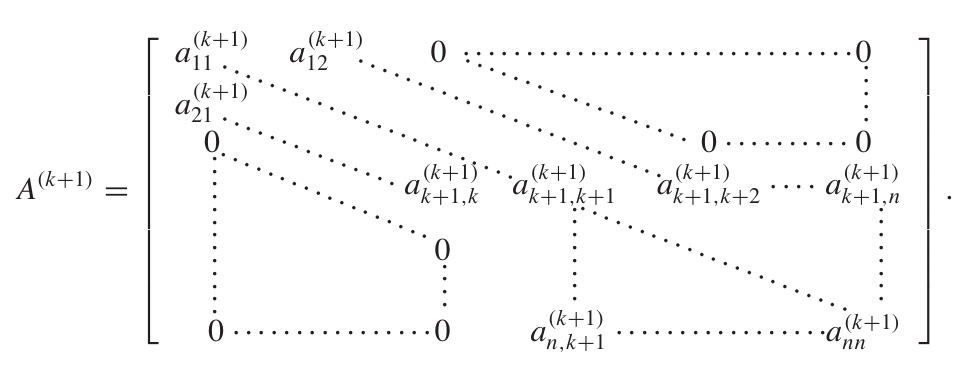
\includegraphics[scale=0.5]{matrizfea.png}
\end{center}



















\singlespacing

\cleardoublepage
\phantomsection % Crea un punto de referencia para el enlace correcto
\addcontentsline{toc}{chapter}{Bibliography}
\bibliography{references}

\end{document}
